\section{Accesso/uscita}
Per poter usufruire delle funzionalità offerte dall'applicazione \Premi è necessario avere un account nel sistema.\\Se l'utente dispone già di un account può accedere al sistema direttamente tramite autenticazione.
\subsection{Registrazione}
Il primo passo per un nuovo utente che decide di utilizzare l'applicazione \Premi consiste nell'effettuare la registrazione.\\Per poter effettuare la registrazione l'utente deve eseguire le seguenti azioni:
\begin{enumerate}
\item Premere il pulsante \textbf{\textit{Registrati}} presente nella parte bassa della casella di autenticazione, in questo modo verrà visualizzata la pagina di registrazione;
\item Inserire un indirizzo e-mail, che verrà utilizzato per identificare l'utente nel sistema;
\item Inserire una password, per proteggere il proprio account;
\item Reinserire la password utilizzata al punto precedente per confermarla;
\item Premere il pulsante \textbf{\textit{Crea account}} per confermare i dati inseriti ed accedere al sistema.
\end{enumerate}
\begin{figure}[H]
\centering
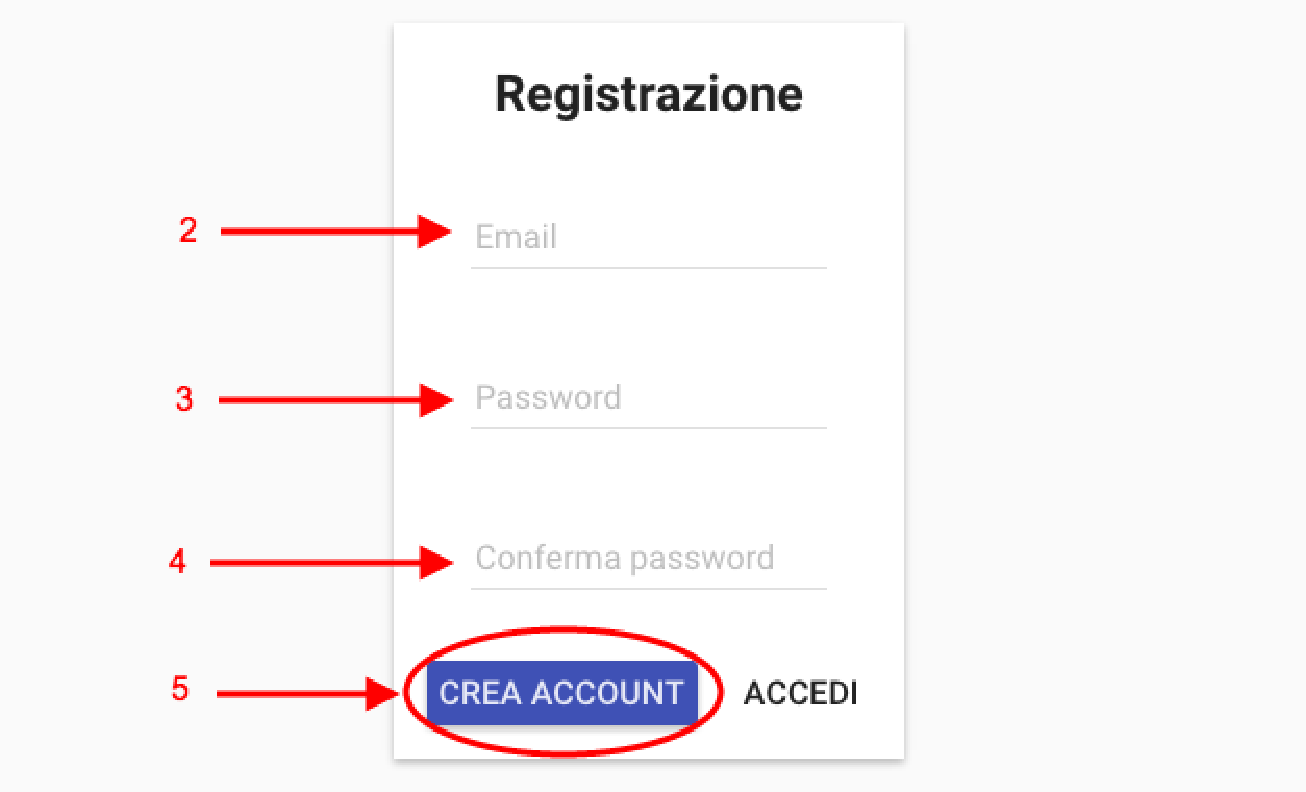
\includegraphics[scale=0.5]{immagini/imgRegistrazione.pdf}
\caption{Form di registrazione}
\end{figure}
%<img src="img/imgRegistrazione.png" alt="imgRegistrazione" width="490" height="440">
Se i dati inseriti non sono corretti o se i campi obbligatori non sono stati compilati verrà visualizzato un messaggio d'errore.
\subsection{Autenticazione}
L'autenticazione permette all'utente di accedere all'applicazione \Premi e di usufruire delle sue funzionalità.\\ Per poter eseguire la procedura di autenticazione l'utente deve aver già effettuato la registrazione al sistema.\\
Per autenticarsi l'utente deve:
\begin{enumerate}
\item Inserire l'indirizzo e-mail utilizzato in fase di registrazione;
\item Inserire la password utilizzata in fase di registrazione;
\item Premere il pulsante \textbf{\textit{Accedi}} per confermare i dati ed accedere al sistema.
\end{enumerate}
\begin{figure}[H]
\centering
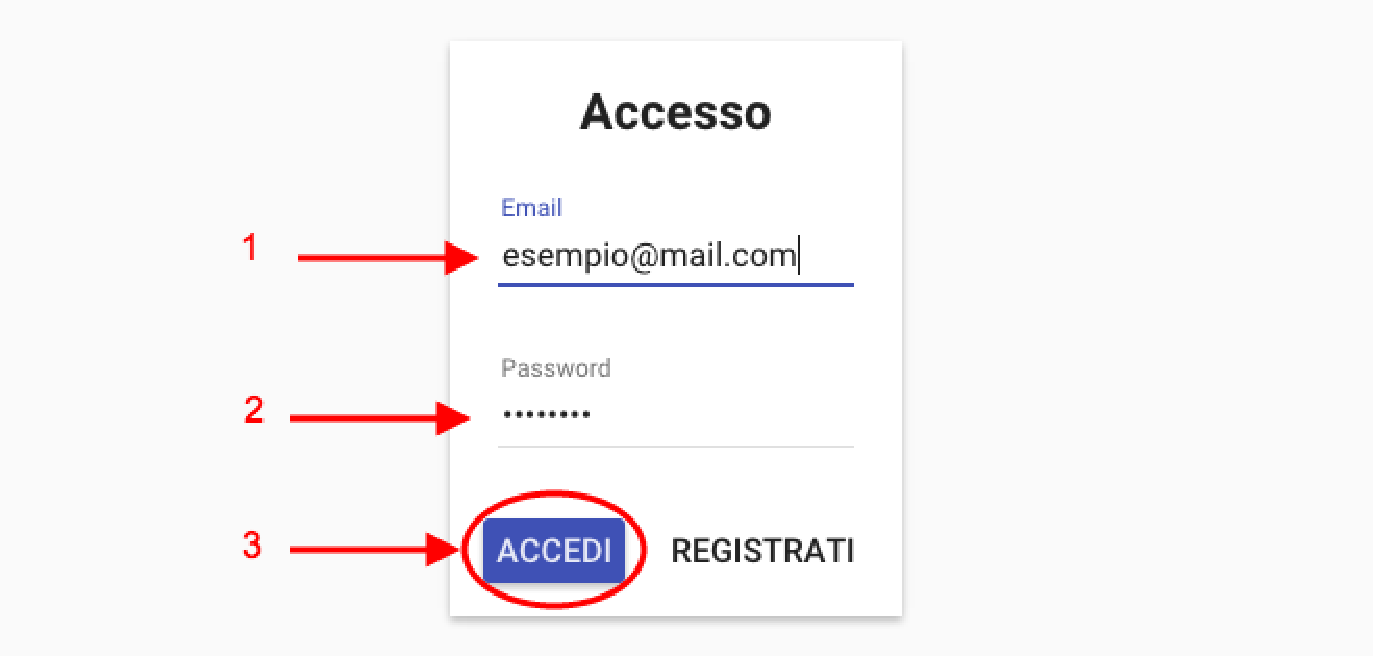
\includegraphics[scale=0.5]{immagini/imgAccesso.pdf}
\caption{Form di accesso}
\end{figure}
%<img src="img/imgAccesso.png" alt="imgAccesso" width="486" height="375">
Se i dati inseriti non sono corretti o se i campi obbligatori non sono stati compilati verrà visualizzato un messaggio d'errore.
\subsection{Uscita}
L'utente può deautenticarsi dal sistema in ogni momento eseguendo la procedura di \textit{Logout}.\\Per effettuare questa procedura l'utente deve trovarsi nella \textit{Dashboard} e premere il pulsante \textbf{\textit{Esci}} presente nella barra di intestazione dell'applicazione .\\
Una volta effettuata la deautenticazione l'utente verrà reindirizzato alla pagina d'accesso dell'applicazione.
\begin{figure}[H]
\centering
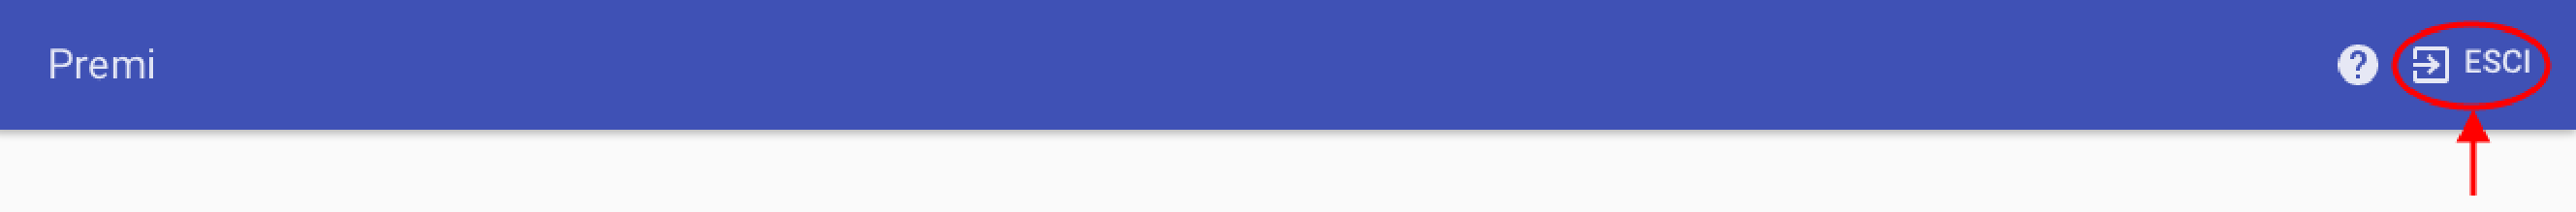
\includegraphics[scale=0.3]{immagini/imgEsci.pdf}
\caption{Pulsante di uscita}
\end{figure}
%<img class="imgLunga" src="img/imgEsci.png" alt="imgEsci" width="1276" height="122">
L'utente può accedere alla \textit{Dashboard} sia dalle pagine dedicate alla modifica del \gloxy{progetto}, sia dalla pagina di presentazione tramite il pulsante \textbf{\textit{Chiudi progetto}} presente all'interno del menu della pagina.
